\documentclass[11pt,a4paper]{article}
\PassOptionsToPackage{obeyspaces,spaces}{url}
\usepackage[T1]{fontenc}
\usepackage[utf8]{inputenc}
\usepackage{lmodern}
\usepackage[margin=2.3cm]{geometry}
\usepackage{xcolor}
\usepackage{listings}
\usepackage{booktabs}
\usepackage{tabularx}
\usepackage{longtable}
\usepackage{xltabular}
\usepackage{array}
\usepackage{amsmath}
\usepackage{tikz}
\usetikzlibrary{arrows.meta,positioning,fit,calc,shapes.geometric,backgrounds}
\usepackage{enumitem}
\usepackage{titlesec}
\usepackage{caption}
\usepackage[most]{tcolorbox}
\usepackage[hidelinks]{hyperref}

\setlength{\parskip}{0.55em}
\setlength{\parindent}{0pt}
\emergencystretch=4em
\setlist{itemsep=0.15em,topsep=0.3em}
\titleformat{\section}{\Large\bfseries}{\thesection.}{0.6em}{}
\titleformat{\subsection}{\large\bfseries}{\thesubsection}{0.6em}{}
\titleformat{\subsubsection}{\normalsize\bfseries}{\thesubsubsection}{0.6em}{}

\definecolor{kw}{HTML}{8A3B12}
\definecolor{cm}{HTML}{6A737D}
\definecolor{st}{HTML}{22863A}
\definecolor{bg}{HTML}{F6F8FA}
\definecolor{attr}{HTML}{005CC5}
\definecolor{boxline}{HTML}{D0D7DE}
\definecolor{noteback}{HTML}{FFF8E5}
\definecolor{noteline}{HTML}{E3B341}

\lstdefinelanguage{Rust}{
  morekeywords={fn,let,mut,pub,const,struct,enum,impl,for,in,while,if,else,match,return,where,use,mod,Some,None,true,false,as,self,Self,type,loop},
  sensitive=true,
  morecomment=[l]{//},
  morecomment=[s]{/*}{*/},
  morestring=[b]",
}
\lstset{
  language=Rust,
  basicstyle=\ttfamily\footnotesize,
  keywordstyle=\color{kw}\bfseries,
  commentstyle=\color{cm}\itshape,
  stringstyle=\color{st},
  backgroundcolor=\color{bg},
  frame=single, rulecolor=\color{boxline}, framerule=0.4pt,
  xleftmargin=0.4em, xrightmargin=0.4em,
  aboveskip=0.6em, belowskip=0.4em,
  breaklines=true, breakatwhitespace=false,
  columns=fullflexible, keepspaces=true,
  showstringspaces=false, tabsize=4,
  literate={->}{{$\rightarrow$}}2 {=>}{{$\Rightarrow$}}2,
}
% Inline code that can break at `_`, `/`, `(`, `,`, `=` and spaces, so long
% identifiers do not overrun the margin.
\usepackage{url}
\DeclareUrlCommand\code{\urlstyle{tt}}
\renewcommand{\UrlBreaks}{\do\_\do\/\do\(\do\[\do\,\do\=\do\:\do\.\do\<\do\-}
\newcommand{\issue}[1]{\textsf{\small #1}}
\newtcolorbox{note}[1][Note]{colback=noteback,colframe=noteline,boxrule=0.5pt,arc=2pt,
  left=6pt,right=6pt,top=4pt,bottom=4pt,fontupper=\small,
  before upper={\textbf{#1.}\ }}

\title{\textbf{The teenygrad Tile DSL}\\[0.4em]
\large Declarations, reverse tile-shape inference worked on conv2d and batch norm,\\
and a Welder schedule for \texttt{conv2d} $\rightarrow$ \texttt{batch\_norm} $\rightarrow$ \texttt{silu}}
\author{}
\date{6 October 2026 \\[0.3em] \small Written against \texttt{feature/anduin-v2} at \texttt{7da014031}, plus PR \#103 (\texttt{9f70215fe})}

\begin{document}
% `#` is an ordinary character in the body, so \code{#[tile]} prints one `#`.
\catcode`\#=12
\maketitle
\thispagestyle{empty}
\vspace{-1em}
\tableofcontents
\newpage

\section{What the DSL is, and what changed since 22 September}

The tile DSL is the set of attributes that \code{#[tiled_kernel]} reads off a kernel's
signature: \code{#[tile(...)]} on parameters, and \code{#[tile_loop]},
\code{#[tile_carry]}, \code{#[tile_reduce_pass]} and \code{#[tile_grid]} on the
function. A single declaration does two different jobs, and almost every subtlety
in this document comes from keeping those two jobs consistent.

\begin{description}[leftmargin=1.2em]
\item[It generates code.] For a kernel whose parameters are \code{In<Tile<T, D>>} /
  \code{Out<Tile<T, D>>} (``route~1''), the macro writes the grid decode, the index
  ranges, the boundary masks, the loads and the output addresses. It can also write
  the accumulation loop, its index decode, the per-iteration operand reads, the
  epilogue and the store (\code{#[tile_loop(generate)]}), or a multi-pass reduction
  followed by a map pass (\code{#[tile_reduce_pass]}). The author writes one
  iteration.
\item[It describes the kernel.] From the same attributes the macro emits
  \code{tile_spec()} (a \code{KernelTileSpec}), \code{grid_spec()} (a
  \code{GridSpec}) and \code{fusion_core()} (an \code{Option<FusionCore>}). These
  are pure data for the scheduler. They answer the question Welder's
  \textsc{Propagate} asks of every node: \emph{if this node's output is tiled this
  way, what tile does each input need?}
\end{description}

A raw-pointer kernel (\code{In<T::Pointer<D>>}, ``route~2'') may also carry
\code{#[tile(...)]}. For it the attributes are metadata only: the body stays
hand-indexed, and only \code{tile_spec()}/\code{grid_spec()} are generated.

\begin{figure}[h]
\centering
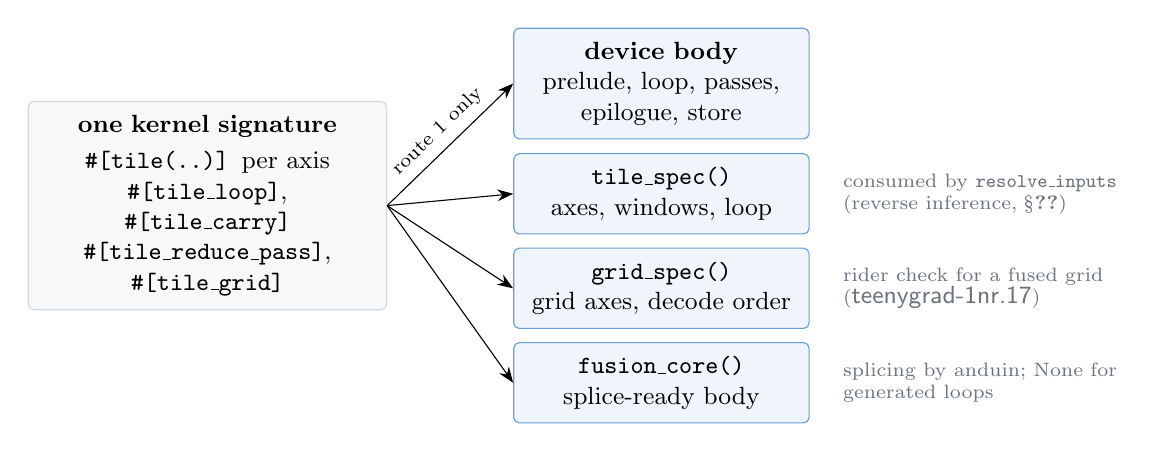
\begin{tikzpicture}[
  box/.style={draw=boxline,fill=bg,rounded corners=2pt,align=center,font=\small,inner sep=5pt},
  prod/.style={draw=attr!60,fill=attr!6,rounded corners=2pt,align=center,font=\small,inner sep=5pt,text width=3.4cm},
  >={Stealth[length=2mm]}]
\node[box,text width=4.2cm] (decl) {\textbf{one kernel signature}\\[2pt]
  \texttt{\#[tile(..)]} per axis\\ \texttt{\#[tile\_loop]}, \texttt{\#[tile\_carry]}\\
  \texttt{\#[tile\_reduce\_pass]}, \texttt{\#[tile\_grid]}};
\node[prod,right=1.6cm of decl,yshift=1.55cm] (pre) {\textbf{device body}\\ prelude, loop, passes,\\ epilogue, store};
\node[prod,right=1.6cm of decl,yshift=0.15cm] (ts) {\textbf{\texttt{tile\_spec()}}\\ axes, windows, loop};
\node[prod,right=1.6cm of decl,yshift=-1.05cm] (gs) {\textbf{\texttt{grid\_spec()}}\\ grid axes, decode order};
\node[prod,right=1.6cm of decl,yshift=-2.25cm] (fc) {\textbf{\texttt{fusion\_core()}}\\ splice-ready body};
\draw[->] (decl.east) -- (pre.west) node[midway,above,sloped,font=\scriptsize]{route 1 only};
\draw[->] (decl.east) -- (ts.west);
\draw[->] (decl.east) -- (gs.west);
\draw[->] (decl.east) -- (fc.west);
\node[font=\scriptsize,align=left,right=0.3cm of ts,text width=3.6cm,text=cm] {consumed by \texttt{resolve\_inputs}\\ (reverse inference, \S\ref{sec:inference})};
\node[font=\scriptsize,align=left,right=0.3cm of gs,text width=3.6cm,text=cm] {rider check for a fused grid (\issue{teenygrad-1nr.17})};
\node[font=\scriptsize,align=left,right=0.3cm of fc,text width=3.6cm,text=cm] {splicing by anduin; \code{None} for generated loops};
\end{tikzpicture}
\caption{One declaration, four products. Because they come from the same tokens, the
code and the metadata cannot drift apart, which is why hand-authored specs are now
forbidden (\S\ref{sec:gotchas}).}
\label{fig:products}
\end{figure}

\subsection{What changed since the 22 September guide}

The previous guide was a field-by-field tour of \code{KernelTileSpec} with a handful
of hand-authored specs and three ``proposed'' features. Most of that has been
overtaken:

{\small
\begin{xltabular}{\linewidth}{>{\raggedright\arraybackslash}p{4.3cm}X}
\toprule
\textbf{Then} & \textbf{Now} \\
\midrule
\endhead
Seven hand-authored \code{const} specs (\code{MATMUL_TILE_SPEC}, \code{CONV1D_TILE_SPEC}, \ldots) at the lowering site. &
All deleted. Every spec is derived by the macro from the kernel's own signature
(\issue{teenygrad-1tl}, about 129 forward kernels converted). \\
\code{TileWindow} declared but not consumed. &
\code{resolve_inputs} computes the receptive field $(b-1)\cdot s+k$. A window carries
\code{output_extent_param} naming the output axis it resolves against, and \code{pad}
is optional (\issue{1nr.18.2}, \issue{1tl.7}). \\
Untiled windowed axes (conv's H) silently dropped. &
They become bindings with the literal block \code{"1"}. \\
\code{TileLoopSpec} proposed. &
Emitted from \code{#[tile_loop]}/\code{#[tile_carry]}. With \code{generate}, the
\emph{macro writes the loop}; \code{init}/\code{finish} give the carry's identity and
the epilogue (\issue{y8aa}, \issue{3dbg}, \issue{3dp5}). \\
Prelude: one flat axis. &
N axes, several blocked axes, broadcast subsets, reduced axes, windowed axes,
\code{fill} values (\issue{1nr.18.1}, \issue{.18.5}, \issue{29qp}, \issue{jpdb}). \\
Row reductions hand-written. &
\code{#[tile_reduce_pass]} with \code{walk} and \code{merge}: declared walks followed by
a generated map pass (\issue{3rk6.2}); the norms are converted. \\
--- &
\code{GridSpec} and \code{#[tile_grid(order|swizzled)]}. \\
\code{FusionCore} a permanent \code{None} stub. &
Revived for single-axis, one-in/one-out, hand-stored kernels (\issue{1cli}, PR \#102). \\
BatchNorm2d lowered with \code{tile_spec: None}. &
\code{#[tile(span = N)]}. BatchNorm2d's spec is rank~4 and attached in the lowering
(\issue{1nr.18.6}, PR \#103). \\
\bottomrule
\end{xltabular}
}

\begin{note}[Scope]
The scheduler side (anduin) has been reset to scaffolding: \code{TileGraph::from_dag}
works, but \code{schedule_graph}, \code{Anduin::schedule}, \code{Trace::trace_graph}
and \code{SimpleProfiler::profile} are \code{todo!()}. The only reverse-inference code
that runs today is the per-node \code{resolve_inputs}
(\code{kernels/teeny-kernels/src/graph/tile_resolve.rs}). The graph-level walk in
\S\ref{sec:inference} and all of \S\ref{sec:welder} describe what that code
\emph{would} do, and say so where it matters.
\end{note}

\section{The attribute vocabulary}
\label{sec:attrs}

All parsing lives in \code{macros/teeny-macros/src/macros/tiled_kernel.rs}. Every
attribute below is host-only metadata: the macro strips it before re-emitting the
device and host signatures, and no attribute macro of that name is registered
anywhere.

\subsection{\texttt{\#[tile(...)]} --- one per real axis, outermost first}

A parameter carries one \code{#[tile(...)]} per axis it declares, in dim order
(dim~0 outermost, NCHW's \code{B} first). The axis's \emph{position} in that list is
its dim index, except that a \code{span} shifts every later index
(\S\ref{sec:span}).

{\small
\begin{xltabular}{\linewidth}{>{\raggedright\arraybackslash}p{3.6cm}>{\raggedright\arraybackslash}X}
\toprule
\textbf{Key} & \textbf{Meaning} \\
\midrule
\endhead
\code{extent = N} \emph{(required)} & The \code{N: i32} runtime parameter giving the axis's total extent. This is the axis's \emph{name} for propagation: two axes anywhere declaring the same extent are the same free variable. \\
\code{block = B} & A \code{const B: i32} generic, or a decimal literal, giving the tile size. Absent means one program per index. A literal (\code{block = 1}) records a kernel that steps the axis one element at a time and has no const to name. \\
\code{name = "B"} & The axis identity for \code{GridSpec} matching, and the suffix of the prelude's index binding (\code{tile_b}). It defaults to the extent's spelling; only \code{conv2d}'s \code{_B} needs it. \\
\code{dim = X|Y|Z} & The hardware grid dimension the axis decodes from. Defaults to \code{X}. \\
\code{window(stride, pad, kernel, output)} & The axis is read through a strided sliding window. \code{stride}/\code{pad}/\code{kernel} are const names or literals, \code{pad} is optional, and \code{output} names the \emph{output} axis the window resolves against. \\
\code{fill = zeros|neg_inf|pos_inf|one|<expr>} & The value of masked lanes: the reduction identity, or \code{constant_pad}'s runtime \code{value}. \\
\code{reduce} (flag) & This tensor is reduced over the axis. At most one per tensor. \\
\code{walk} (flag) & The axis is neither gridded nor loaded whole. A reduce pass or the map pass walks it in \code{block}-sized steps. \\
\code{span = N} & The axis covers \code{N} real dims, flattened row-major. Metadata only. Not allowed with \code{window}, \code{reduce}, or on a single-axis kernel (\S\ref{sec:span}). \\
\bottomrule
\end{xltabular}
}

Rules the macro enforces on route~1. Each is a compile error naming the offending
parameter.
\begin{itemize}
\item Either every \code{Tile} parameter declares \code{#[tile]} or none does. With
  none, the kernel falls back to the implicit \code{BLOCK_SIZE}/\code{n_elements}
  flat convention \emph{and no \code{tile_spec()} is generated}. Because that
  fallback is silent, \code{tests/test_tile_declarations.rs} parses the source to
  catch it.
\item There must be an \code{Out<Tile<..>>}, and it must carry a blocked axis. The
  output's axes are what the grid covers and what every input resolves against.
\item Every input axis must either match an output axis by \code{(extent, block,
  dim)}, be \code{reduce}, or carry a \code{window} whose \code{output} names an
  output axis. An input may declare a \emph{subset} of the output's axes; that is a
  broadcast operand (\S\ref{sec:prelude}).
\item A kernel cannot mix tagged \code{Tile} parameters with tagged raw pointers.
\end{itemize}

\subsection{Per-iteration reads: \texttt{\#[tile\_loop\_tile]} and \texttt{\#[tile\_loop\_scalar]}}

A loop-indexed operand cannot use the prelude's load-once read. Two
parameter attributes declare how it is read \emph{inside} the generated loop
instead. Both apply only to \code{In<Tile<..>>}.

\begin{description}[leftmargin=1.2em,style=nextline]
\item[{\code{#[tile_loop_tile(index = [coord = extent, ..], bounds = [i, ..])]}}]
  Reads a whole tile per iteration at loop-dependent coordinates. Each \code{index}
  entry is a full coordinate \emph{expression} and the layout extent, outermost
  first. The offset is the row-major fold of those pairs. \code{bounds} lists the
  positions whose coordinate gets a \code{ge(0) & lt(extent)} check (the padded
  axes). The coordinates are expressions rather than names on purpose: a windowed
  coordinate mixes a grid index, a loop index and two consts, and inferring which
  loop axis pairs with which window would be ambiguous. Requires exactly one
  blocked output axis.
\item[{\code{#[tile_loop_scalar(index = [idx = extent, ..])]}}]
  Reads one element per iteration at a loop-dependent flat index and broadcasts it
  to the carry's shape. This is conv2d's weight.
\end{description}

A loop-indexed operand still appears in the spec through its \code{#[tile]}
attributes. The two jobs are separate: \code{#[tile]} says what the operand
\emph{is}, and \code{#[tile_loop_tile]} says how to read it.

\subsection{Function attributes}

{\small
\begin{xltabular}{\linewidth}{>{\raggedright\arraybackslash}p{4.4cm}>{\raggedright\arraybackslash}X}
\toprule
\textbf{Attribute} & \textbf{Meaning} \\
\midrule
\endhead
\code{#[tile_loop(trip_count = [..])]} & An accumulation loop. \code{trip_count} is a list of \emph{names}, not a formula. It becomes \code{TileLoopSpec::trip_count_factors}. \\
\quad\code{axes = [name = extent, ..]} & The loop's own axes. Their extents multiply to the trip count, and the generated decode binds each name (innermost first). \\
\quad\code{count = <expr>} & An evaluable trip count, when there are no axes. \\
\quad\code{generate} (flag) & The macro emits the carry init, the loop around the author's body, and the store after it. \\
\code{#[tile_carry(acc = [shape])]} & A loop-carried accumulator. Each shape entry is a const name or a literal. \\
\quad\code{init = <expr>} & Replaces \code{zeros}. Max-pool uses $-\infty$. Requires \code{generate}. \\
\quad\code{finish = <expr>} & The epilogue: \code{let acc = <expr>;} between the loop and the store. Requires \code{generate}. \\
\code{#[tile_reduce_pass(over, read, into, acc, finish?, store?, fill?, merge?)]} & One walk over a \code{walk} axis accumulating into a scalar carry, then \code{finish} and an optional store. Passes run in declaration order. \code{merge} shares the previous pass's walk and read. \\
\code{#[tile_grid(order = [..])]} & The real grid decode order when it differs from the output's dim order, or a subset when a loop covers an axis. \\
\code{#[tile_grid(swizzled)]} & No \code{GridSpec} at all: the decode is not mixed-radix (matmul's \code{GROUP_M}). \\
\bottomrule
\end{xltabular}
}

Errors the loop attributes guard against:
\begin{itemize}
\item a carry without a loop;
\item a loop without a carry (``an independent walk belongs in the grid'');
\item \code{generate} with neither \code{axes} nor \code{count};
\item \code{finish}/\code{init} without \code{generate} (otherwise the expression is silently dropped);
\item \code{generate} with more than one carry or more than one \code{Out<Tile>} (flash attention's three carries need a carry-to-output pairing that does not exist yet);
\item a \code{merge} pass whose \code{read}/\code{over} differs from its leader's.
\end{itemize}

\subsection{\texttt{span}: one declared axis, several real dims}
\label{sec:span}

New in PR \#103. A kernel may address several real dims as one row-major
flattened axis. \code{batch_norm_2d_nchw_forward_inference} walks an NCHW tensor
as \code{[B, C, HW]}. \code{span = 2} tells the spec the truth about the tensor
without touching the body:

\begin{lstlisting}
#[tile(extent = B, dim = Y)]
#[tile(extent = C)]
#[tile(block = BLOCK_HW, extent = HW, span = 2)]   // dims 2 and 3
x: In<Tile<T, D>>,
\end{lstlisting}

Only the metadata moves. The spec's rank is $\sum \text{span}$ (4 here), the
binding's \code{dims} are \code{[2, 3]}, and \code{reduction_axis} is now a real dim
index rather than a declaration position. The prelude still decodes and addresses
one \code{HW} axis. The combinations that would need a meaning the spec types cannot
carry are refused:
\begin{itemize}
\item \code{window}: a window relates one input dim to one output dim.
\item \code{reduce}: \code{reduction_axis} holds a single index.
\item A single-axis kernel: its \code{tile_spec(rank)} already flattens every dim.
\end{itemize}

\section{What the macro generates (route 1)}
\label{sec:prelude}

The metadata in \S\ref{sec:spec} is only trustworthy if it describes the code that
actually runs. This section is that code, taken from the source snapshots in
\code{kernels/teeny-kernels/tests/snapshots/} and reformatted.

\subsection{The prelude}

For the output's axes, outermost first, the prelude emits the following:
\begin{enumerate}
\item \textbf{A mixed-radix grid decode.} One \code{program_id} per hardware dim is
  decoded innermost-first. A blocked axis counts \code{cdiv(extent, block)} programs
  and an unblocked one counts \code{extent}. The outermost axis takes the remainder.
  Each axis gets an index \code{tile_<name>}. For a blocked axis that is the
  \emph{tile} index, not an element offset.
\item \textbf{A range per blocked axis.} The range is \code{arange(0, B) + tile_x * B},
  named \code{__tile_range}, or \code{__tile_range_<slot>} broadcast to the full
  K-D tile shape when several axes are blocked.
\item \textbf{A mask.} \code{in_bounds} is the conjunction of
  \code{range.lt(extent)} over the blocked axes.
\item \textbf{Row-major offsets.} Strides are derived from the declared extents.
  The blocked range is a tensor term and every unblocked index a scalar term, summed
  \emph{tensor first}, because only \code{Tensor + i32} has an impl.
\item \textbf{Per input,} a \emph{loaded} \code{Tile { tensor, mask }}:
  \begin{itemize}
  \item A \textbf{broadcast} operand (a subset of the output's axes) loads its one
    element and \code{broadcast_to}s the tile shape, with no mask.
  \item A \textbf{reduced} axis gets its own \code{arange(0, BLOCK)} masked to its
    extent, with no \code{+ pid * BLOCK}. Every program reads it in full.
  \item A \textbf{windowed} axis reads the shifted coordinate
    \code{base * stride - pad}, bounds-checked against its own extent.
  \end{itemize}
\item \textbf{Per output,} an \emph{addressed} \code{Tile}, whose \code{.tensor} is the
  pointer tensor \code{y.add_offsets(offsets)}. The body stores through it.
\end{enumerate}

\subsection{conv2d\_forward, fully expanded}

The whole author-written body of \code{conv2d_forward} is one line,
\code{acc = acc + x * w;}. Everything below is generated. This is from
\code{test_conv2d__conv2d_forward_source_cuda.snap}, with the \code{where} clause
and entry point elided:

\begin{lstlisting}
// -- prelude: decode (b, c_out, oh, ow_tile), innermost first
let mut __tile_rem_x = T::program_id(Axis::X);
let tile_ow    = __tile_rem_x % T::cdiv(OW, BLOCK_OW); __tile_rem_x /= T::cdiv(OW, BLOCK_OW);
let tile_oh    = __tile_rem_x % OH;                    __tile_rem_x /= OH;
let tile_c_out = __tile_rem_x % C_OUT;                 __tile_rem_x /= C_OUT;
let tile_b     = __tile_rem_x;
let __tile_range = T::arange(0, BLOCK_OW) + tile_ow * BLOCK_OW;
let in_bounds    = __tile_range.lt(OW);
let offsets = __tile_range + tile_b * (C_OUT * OH * OW) + tile_c_out * (OH * OW) + tile_oh * OW;
let y = Tile::<T, T::Pointer<D>> { tensor: y.add_offsets(offsets), mask: Some(in_bounds) };
// x and w are loop-indexed: no prelude load.

// -- #[tile_loop(generate)] + #[tile_carry(acc = [BLOCK_OW])]
let mut acc = T::zeros::<D>(&[BLOCK_OW]);
for __tile_loop_idx in 0..((C_IN / G) * KH * KW) {
    // decode the loop axes [c_in_local = C_IN/G, kh = KH, kw = KW], innermost first
    let mut r = __tile_loop_idx;
    let kw = r % KW; r = r / KW;
    let kh = r % KH; r = r / KH;
    let c_in_local = r;
    // #[tile_loop_scalar]: one weight element, broadcast to the carry
    let w = T::broadcast_to(T::load(w.add_offsets(T::arange(0, 1)
              + (kw + (kh + (c_in_local + tile_c_out * (C_IN / G)) * KH) * KW)), ..), &[BLOCK_OW]);
    // #[tile_loop_tile]: a windowed row of x, masked on H and W (bounds = [2, 3])
    let x = {
        let ih = __tile_range * 0 + (tile_oh * STRIDE_H + kh - PAD_H);  // scalar, splatted
        let iw = __tile_range * STRIDE_W + kw - PAD_W;                   // tensor
        let m  = in_bounds & (ih.ge(0) & ih.lt(H)) & (iw.ge(0) & iw.lt(W));
        T::load(x.add_offsets(iw + (ih + (((tile_c_out / (C_OUT / G)) * (C_IN / G)
                + c_in_local) + tile_b * C_IN) * H) * W), Some(m), Some(T::zeros(&[BLOCK_OW])), ..)
    };
    acc = acc + x * w;                       // <- the author's body
}
T::store(y.tensor, acc, Some(in_bounds), ..);  // generated store
\end{lstlisting}

Three facts in this expansion matter for scheduling:
\begin{itemize}
\item \textbf{One program computes a $1\times1\times1\times\text{BLOCK\_OW}$ strip.} Only
  \code{OW} is blocked, and \code{B}, \code{C_OUT}, \code{OH} are one-per-program.
  Changing the program's tile along any other axis means changing the declaration
  and therefore the body. No consumer can just ``choose'' it.
\item \textbf{The reduction is walked one element at a time.} The loop steps through
  every \code{(c_in, kh, kw)}. There is no reduction chunk (Welder's \code{rstep}) to
  tune.
\item \textbf{The per-iteration read of \code{x} spans
  $(\text{BLOCK\_OW}-1)\cdot \text{STRIDE\_W}+1$ columns,} and across the \code{kw}
  iterations
  $(\text{BLOCK\_OW}-1)\cdot\text{STRIDE\_W}+\text{KW}$ columns: exactly the window
  the spec declares.
\end{itemize}

\subsection{Reduce passes and the map pass}

\code{#[tile_reduce_pass]} turns a multi-pass kernel into declarations plus one
author-written map pass:
\begin{itemize}
\item Each pass group emits a \code{while} over its \code{walk} axis in
  \code{block}-sized steps. A walk axis that is not innermost advances by the product
  of the extents inside it.
\item The group loads \code{read} once per step and adds each pass's \code{acc} into
  its scalar carry. A \code{merge} pass joins the previous walk, so one read feeds
  several carries.
\item After the walk come the \code{finish}es and \code{store}s, in declaration
  order. A later \code{finish} may therefore name an earlier carry.
\item Then comes either the \textbf{map pass} or a \textbf{reduce-only} tail. The map
  pass is a second walk over the \emph{output's} walked axis: it loads every walked
  input, evaluates the author's body as an expression, and stores it. In a
  reduce-only kernel the body simply runs after the walks. That is
  \code{batch_norm_stats_forward}.
\end{itemize}

\code{batch_norm_stats_forward}'s generated body
(\code{test_batchnorm__batch_norm_stats_source_cuda.snap}):

\begin{lstlisting}
let pid = T::program_id(Axis::X); let tile_c = pid;             // single-axis prelude, grid [C]
let offsets = T::arange(0, 1) + pid * 1; let in_bounds = offsets.lt(C);
let mean = Tile { tensor: mean.add_offsets(offsets), mask: Some(in_bounds) };
let rstd = Tile { tensor: rstd.add_offsets(offsets), mask: Some(in_bounds) };
let mut sum = T::zeros::<D>(&[1]); let mut sum_sq = T::zeros::<D>(&[1]);
let mut n0: i32 = 0;
while n0 < N {                                       // ONE walk for both passes (merge)
    let col = T::arange(0, BLOCK_N) + n0; let m = col.lt(N);
    let x = T::load(x.add_offsets(col * C + tile_c), Some(m), Some(T::zeros(&[BLOCK_N])), ..);
    sum    = sum    + T::sum(x, None, true);
    sum_sq = sum_sq + T::sum(x * x, None, true);
    n0 += BLOCK_N;
}
let sum = sum * (1/N);                 T::store(mean.tensor, sum, ..);   // pass 1 finish + store
let sum_sq = sum_sq * (1/N) - sum * sum;                                 // pass 2 finish: variance
// ... the author's body: rstd = rsqrt(var + eps), running-stat EMA updates
\end{lstlisting}

The \code{x} axis \code{N} is declared \code{reduce, walk}. Note the offset
\code{col * C + tile_c}: \code{N} is the \emph{outer} axis of an \code{[N, C]} tensor,
so each walk step advances by \code{C}. This kernel views its input as 2-D
\code{[N, C]}, which matters in \S\ref{sec:bn-train}.

\subsection{Epilogues: \texttt{finish}}

\code{finish} is the slot between the loop and the store, and it is how the fused
\code{conv2d_bn_silu_forward} is written. The kernel is the conv2d declaration
verbatim, plus:

\begin{lstlisting}
#[tile_carry(
    acc = [BLOCK_OW],
    finish = {
        let bn_off = T::arange(0, 1) + tile_c_out;           // per-channel, from the grid decode
        let scale = T::broadcast_to(T::load(bn_scale_ptr.add_offsets(bn_off), ..), &[BLOCK_OW]);
        let shift = T::broadcast_to(T::load(bn_shift_ptr.add_offsets(bn_off), ..), &[BLOCK_OW]);
        let bn_out = scale * acc + shift;                       // BatchNorm (prefolded)
        let one = T::full(&[BLOCK_OW], 1.0_f32); let neg1 = T::full(&[BLOCK_OW], -1.0_f32);
        bn_out * (one / (one + T::exp(neg1 * bn_out)))          // SiLU
    }
)]
\end{lstlisting}

\S\ref{sec:welder} argues that this \code{finish} slot is exactly where a Welder-style
register-level connection lands in this DSL.

\section{What the macro describes: the spec types}
\label{sec:spec}

\subsection{The types (\texttt{core/teeny-core/src/model/tile\_spec.rs})}

\begin{lstlisting}
KernelTileSpec   { inputs: &[TensorTileSpec], outputs: &[TensorTileSpec], loop_spec: Option<TileLoopSpec> }
TensorTileSpec   { param, rank, axes: &[TileAxisBinding], reduction_axis: Option<usize>, untiled_dims: &[&str] }
TileAxisBinding  { dims: &[usize], block_const, extent_param, window: Option<TileWindow>, divide_by: Option<usize> }
TileWindow       { output_extent_param, stride_const, pad_const: Option<&str>, kernel_size_const }
TileLoopSpec     { carries: &[TileCarryBinding], trip_count_factors: &[&str] }
TileCarryBinding { name, shape_consts: &[&str] }            // entries: const names or "1"
\end{lstlisting}

There are still no enums and no variants. Every ``case'' is a combination of field
values. Every string is a \emph{name}, never a value: the spec has no per-node
parameter lookup, so a consumer that needs numbers must be given a
\code{ConstLookup} by its caller. \code{KernelTileSpec::validate()} checks the
invariants the types cannot hold:
\begin{itemize}
\item dims are below the rank and appear at most once;
\item no name is both bound and untiled;
\item there are no more described dims than the rank;
\item every carry has a shape;
\item there is at least one output, unless the spec is loop-only.
\end{itemize}

\subsection{How a declaration becomes a binding}

The same per-axis rule applies on both routes:

{\small
\begin{xltabular}{\linewidth}{>{\raggedright\arraybackslash}p{4.8cm}X}
\toprule
\textbf{Declared axis} & \textbf{Emitted} \\
\midrule
\endhead
\code{block = B} (not \code{walk}) & A \code{TileAxisBinding { dims, block_const: "B", extent_param, window }} \\
\code{block = B, walk} & \emph{No binding}; its name goes to \code{untiled_dims}. One program walks the whole axis, so it cannot be split across programs. A binding would tell the scheduler it can be. \\
no \code{block}, with \code{window(..)} & A binding with the literal \code{block_const: "1"}, so the window has something to hang off. \\
no \code{block}, no window & No binding; the name goes to \code{untiled_dims}. \\
\code{reduce} & Sets \code{reduction_axis} to the axis's real dim. \\
\code{span = N} & \code{dims} is the next \code{N} real dims; the rank grows by $N-1$. \\
\bottomrule
\end{xltabular}
}

Which parameters appear, and with what rank:
\begin{itemize}
\item \textbf{Route 1, several declared axes:} \code{tile_spec()} at a \emph{fixed}
  rank. Each parameter reports its own axes, so a \code{(C,)} bias against an
  \code{[N, C]} output is rank~1 (\issue{1tl.4}).
\item \textbf{Route 1, one flat axis:} \code{tile_spec(rank)}, with one binding over
  \code{dims = [0..rank)}. The same flat kernel applies at any rank, so the graph node
  supplies it. The lowering calls \code{SiluForward::<f32>::tile_spec(node.shape.len())}.
\item \textbf{Route 2:} \code{tile_spec()} at fixed rank. \code{InOut} parameters
  appear in both lists.
\item \textbf{Loop only:} flash attention declares its loop and no tensors
  (\code{BH} is a grid extent, not a parameter), so it gets a spec with empty
  \code{inputs}/\code{outputs}. \code{validate()} accepts it; \code{resolve_inputs}
  rejects it.
\item \textbf{An input with no \code{#[tile]} is omitted from the spec entirely.}
  conv2d's weight is the important case: its second extent is \code{C_IN / G},
  which \code{extent = <ident>} cannot name. It is read through
  \code{#[tile_loop_scalar]} and does not appear in the spec.
\end{itemize}

\subsection{GridSpec and FusionCore}

\code{grid_spec()} lists the output's non-walked axes as \code{GridAxisBinding { name,
extent_factors, dim, block_const }}, in dim order. If a \code{#[tile_grid(order =
..)]} is present it uses that order and subset instead. For example:
\begin{itemize}
\item \code{transpose_2d_forward} decodes \code{M} outer while its output is
  \code{[N, M]}.
\item \code{batch_norm_normalize_forward}'s grid is \code{[C]} alone.
\item \code{conv2d_bn_silu_tiled} decodes \code{(B, OH, C_OUT, OW)}.
\end{itemize}
\code{swizzled} emits no grid spec at all. The purpose is the ``rider'' check of
\issue{teenygrad-1nr.17}: a fused op can reuse the anchor's already-decoded indices
only if its grid axes are a name-matching subset of the anchor's.

\code{fusion_core()} returns \code{Some(FusionCore { input_ident, output_ident,
body_source, extra_params })} (the body minus its trailing store) only when all of
these hold:
\begin{itemize}
\item exactly one \code{In<Tile>} and one \code{Out<Tile>};
\item each declares one axis;
\item the hand-written body ends in \code{T::store(..)};
\item there is no \code{generate} loop and no loop-indexed operand.
\end{itemize}
\code{silu_forward} qualifies. \code{batch_norm_2d_nchw_forward_inference} (five
inputs) and \code{conv2d_forward} (generated loop) do not. Whether a generated-loop
kernel even \emph{has} a fusion core is recorded as undecided in
\issue{teenygrad-1cli}. \S\ref{sec:welder-infer} proposes an answer.

\section{Reverse tile-shape inference}
\label{sec:inference}

\subsection{The question, and the two halves of the answer}

Welder's \textsc{Propagate} starts from a chosen \emph{output} tile and walks the
graph backwards. At each node it asks which region of each input the tile needs.
Two separate mechanisms answer this:

\begin{enumerate}
\item \textbf{Within a node:} \code{resolve_inputs(spec, output_tile, consts)} in
  \code{kernels/teeny-kernels/src/graph/tile_resolve.rs}. This is a pure function
  that is fully implemented and tested.
\item \textbf{Across an edge:} the input tile a consumer needs becomes the output
  tile its producer must supply. This is the graph walk. It is not implemented
  today (\code{TileGraph} has only \code{from_dag}). \S\ref{sec:edges} describes what
  it must do and where the DSL makes that hard.
\end{enumerate}

A tile is a \code{TileShape = Vec<Option<usize>>}: one entry per \emph{real} dim,
with \code{None} meaning ``unresolved, therefore full extent''.

\subsection{\texttt{resolve\_inputs}, step by step}

\begin{lstlisting}
fn resolve_inputs(spec, output_tile, consts) -> Result<Vec<TileShape>> {
    let out = spec.outputs[0];                     // error if there are no outputs
    require output_tile.len() == out.rank;          // error otherwise -- the BN2d trap, Sec. 7
    // 1. read the blocks the output was given, keyed by NAME
    let resolved = for axis in out.axes:
        block = product of output_tile[d] for d in axis.dims   // None if any is None
        if block is Some: (axis.extent_param, block)
    // 2. for each input, start all-None and place only what can be placed
    for input in spec.inputs:
        tile = [None; input.rank]
        for axis in input.axes:
            name  = axis.window.map(|w| w.output_extent_param).unwrap_or(axis.extent_param)
            block = match resolved.get(name) {
                Some(b) => b,
                None if axis.window.is_some() => continue,         // stays full extent
                None => consts.get(axis.extent_param) / divide_by, // or continue
            };
            extent = match axis.window {
                None => block,
                Some(w) => (block - 1) * stride(w) + kernel(w),    // receptive field; or continue
            };
            tile[last of axis.dims] = extent;  tile[other dims] = 1;  // product-preserving
        yield tile
}
\end{lstlisting}

The rules, each of which has a test in \code{tile_resolve.rs}:

\begin{description}[leftmargin=1.2em]
\item[Names, not arithmetic.] An input axis takes the block of the output axis with
  the same \code{extent_param}. GEMM's \code{a}/\code{c} both name \code{M}, and
  transpose's permuted axes resolve by name regardless of position. An axis whose
  name the output never declares, such as GEMM's \code{K}, stays \code{None}. That
  is correct, because a reduction axis is the search's to choose, not the output's.
\item[Unresolved means full extent.] This is the conservative direction: an
  over-estimate is safe against a hard memory capacity, and an under-estimate is
  not. It covers three cases:
  \begin{itemize}
  \item an axis with no binding (untiled, walked or reduced);
  \item an unmatched name;
  \item a window whose consts the caller did not supply.
  \end{itemize}
\item[Windows invert by the receptive field.] A windowed input axis resolves against
  the \emph{output} variable its window names (\code{OW}), not its own extent
  (\code{W}). The tile is then $(b-1)\cdot s + k$. Padding shifts the origin, not
  the size, so it never enters. The pad family is the degenerate window
  $s=k=1$, whose tile is $b$.
\item[A window never takes the full-extent fallback through the window.] Feeding
  \code{H} through $(H-1)s+k$ would claim the kernel reads past the tensor. An
  unresolved windowed axis therefore stays \code{None}.
\item[Only the output's \emph{bound} axes seed anything.] The output tile has a value
  in every dim, but \code{resolve_inputs} reads only the dims covered by
  \code{out.axes}. A value at an untiled output dim (\code{B}, \code{C_OUT},
  \code{OH} for conv2d) is ignored. This single rule produces conv2d's large
  over-estimate (\S\ref{sec:conv-overestimate}).
\item[Flattened bindings are product-preserving.] The block lands on the innermost
  dim of \code{axis.dims} and the others become \code{1}. Reading a flattened
  \emph{output} binding multiplies its dims back together, so the two directions are
  inverse \emph{on the product}. They are not an axis-aligned region once the block
  exceeds the innermost extent (\S\ref{sec:edges}).
\item[\texttt{divide\_by} replaces a full extent.] It is applied only on the
  \code{consts} fallback path, never to a propagated block. The macro always emits
  \code{None}, because GroupNorm's \code{C / G} is per-instance
  (\issue{1nr.15}).
\end{description}

\subsection{Crossing an edge}
\label{sec:edges}

The resolved input tile is in the consumer's \emph{dim coordinates}. The producer's
\code{resolve_inputs} needs an output tile in \emph{its} dim coordinates. Names do
not help across an edge: conv2d's output calls its axes \code{B/C_OUT/OH/OW},
BatchNorm2d's input \code{B/C/HW}, and SiLU's \code{n_elements}. The only shared
coordinate system is the tensor's real dims, so the walk must pass \code{TileShape}s
\emph{by position}. That imposes three requirements on the DSL.

\begin{enumerate}
\item \textbf{Ranks must agree.} A kernel whose view of a tensor has a different rank
  from the edge cannot take part. That was BatchNorm2d before \code{span}.
\item \textbf{Full extent must be materialised.} \code{None} on the consumer side
  means ``all of it''. The producer must read that as the real extent, which comes
  from the node's shape, not as ``unconstrained''.
\item \textbf{Flattened tiles must be re-expressed axis-aligned, or the producer will
  misread them.} SiLU's flat spec turns an output tile into \code{[1, 1, 1, 1024]}.
  BatchNorm2d's spanned \code{HW} passes that on as \code{[_, _, 1, 1024]}. Handed to
  conv2d as an output tile, that says ``1024 columns of \code{OW}'' on a tensor 32
  wide. The honest translation is \code{[_, _, 32, 32]} (32 rows of 32). Welder's own
  implementation clamps every propagated region to the producer's real shape
  (\code{graph.py}, \code{propogate_inputs}), and a teenygrad walk needs at least
  that clamp. It also needs the reshape from a product to an axis-aligned box
  whenever the block exceeds the innermost extent.
\end{enumerate}

\begin{note}[A useful invariant]
A flattened block $b$ over dims $(\ldots, H, W)$ is an axis-aligned
$\lceil b/W\rceil \times \min(b, W)$ box exactly when $b \le W$ and $W \bmod b = 0$,
or when $W \mid b$. For BatchNorm2d's \code{BLOCK_HW = 128} on a $32\times32$ plane,
that is a $4\times32$ box. A walk can convert under this condition and fall back to
full extent otherwise.
\end{note}

\section{Worked kernel: conv2d}
\label{sec:conv2d}

\subsection{The declaration, axis by axis}

\begin{lstlisting}
#[tiled_kernel]
#[tile_loop(trip_count = [C_IN, G, KH, KW],
            axes = [c_in_local = (C_IN / G), kh = KH, kw = KW], generate)]
#[tile_carry(acc = [BLOCK_OW])]
pub fn conv2d_forward<T: Triton, D: Num, const KH: i32, const KW: i32,
    const STRIDE_H: i32, const STRIDE_W: i32, const PAD_H: i32, const PAD_W: i32,
    const G: i32, const BLOCK_OW: i32>(
    #[tile(name = "B", extent = _B)]                                     // dim 0: untiled
    #[tile(extent = C_IN)]                                               // dim 1: untiled
    #[tile(extent = H, window(stride = STRIDE_H, pad = PAD_H, kernel = KH, output = OH))]
    #[tile(block = BLOCK_OW, extent = W,
           window(stride = STRIDE_W, pad = PAD_W, kernel = KW, output = OW))]
    #[tile_loop_tile(index = [tile_b = _B,
        ((tile_c_out / (C_OUT / G)) * (C_IN / G) + c_in_local) = C_IN,
        (tile_oh * STRIDE_H + kh - PAD_H) = H,
        (__tile_range * STRIDE_W + kw - PAD_W) = W], bounds = [2, 3])]
    x: In<Tile<T, D>>,
    #[tile_loop_scalar(index = [tile_c_out = C_OUT, c_in_local = (C_IN / G), kh = KH, kw = KW])]
    w: In<Tile<T, D>>,                                                   // no #[tile]: not in spec
    #[tile(name = "B", extent = _B)]
    #[tile(extent = C_OUT)]
    #[tile(extent = OH)]
    #[tile(block = BLOCK_OW, extent = OW)]
    y: Out<Tile<T, D>>,
    _B: i32, C_IN: i32, C_OUT: i32, H: i32, W: i32, OH: i32, OW: i32,
) { acc = acc + x * w; }
\end{lstlisting}

\begin{itemize}
\item \textbf{\code{x}'s H and W axes} name their own extents (\code{H}, \code{W}) and,
  through \code{output = OH/OW}, the output variable they resolve against. Naming the
  input axis \code{OW} would also resolve, but the spec would then claim the input's
  width \emph{is} \code{OW}, which \code{untiled_dims} and any footprint model would
  believe.
\item \textbf{The input and output axes match through windows.} The prelude check
  (``every input axis matches an output axis'') is satisfied by the windows. \code{x}
  is loop-indexed, so the prelude does not place it anyway.
\item \textbf{\code{#[tile_loop_tile]} restates the coordinates as expressions.} The
  window says \emph{what} is read; the index list says \emph{where}. They have to
  agree, and nothing checks that they do (\S\ref{sec:gotchas}).
\end{itemize}

\subsection{What \texttt{tile\_spec()} and \texttt{grid\_spec()} return}

\begin{lstlisting}
KernelTileSpec {
  inputs: [ TensorTileSpec { param: "x", rank: 4, reduction_axis: None,
              untiled_dims: ["B", "C_IN"],
              axes: [ { dims: [2], block_const: "1",        extent_param: "H",
                        window: Some({ output: "OH", stride: "STRIDE_H", pad: Some("PAD_H"), kernel: "KH" }) },
                      { dims: [3], block_const: "BLOCK_OW", extent_param: "W",
                        window: Some({ output: "OW", stride: "STRIDE_W", pad: Some("PAD_W"), kernel: "KW" }) } ] } ],
  outputs: [ TensorTileSpec { param: "y", rank: 4, reduction_axis: None,
              untiled_dims: ["B", "C_OUT", "OH"],
              axes: [ { dims: [3], block_const: "BLOCK_OW", extent_param: "OW", window: None } ] } ],
  loop_spec: Some(TileLoopSpec { carries: [{ name: "acc", shape_consts: ["BLOCK_OW"] }],
                                 trip_count_factors: ["C_IN", "G", "KH", "KW"] }),
}
GridSpec { axes: [ B(_B), C_OUT, OH, OW(BLOCK_OW) ] }      // all on GridDim::X, in decode order
\end{lstlisting}

\subsection{Resolving it}

\begin{figure}[h]
\centering
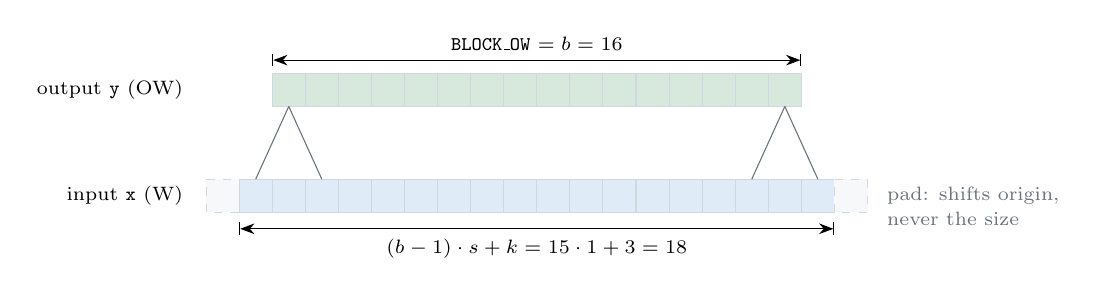
\begin{tikzpicture}[x=0.42cm,y=0.42cm,>={Stealth[length=1.8mm]}]
  % input row
  \foreach \i in {0,...,17} { \draw[fill=attr!12,draw=boxline] (\i,0) rectangle ++(1,1); }
  \foreach \i in {-1,18} { \draw[fill=bg,draw=boxline,dashed] (\i,0) rectangle ++(1,1); }
  \node[font=\scriptsize,anchor=east] at (-1.4,0.5) {input \texttt{x} (W)};
  % output row
  \foreach \i in {0,...,15} { \draw[fill=st!18,draw=boxline] (\i+1,3.2) rectangle ++(1,1); }
  \node[font=\scriptsize,anchor=east] at (-1.4,3.7) {output \texttt{y} (OW)};
  % window lines for first and last output
  \draw[color=cm] (1.5,3.2) -- (0.5,1); \draw[color=cm] (1.5,3.2) -- (2.5,1);
  \draw[color=cm] (16.5,3.2) -- (15.5,1); \draw[color=cm] (16.5,3.2) -- (17.5,1);
  \draw[|<->|] (1,4.6) -- (17,4.6) node[midway,above,font=\scriptsize] {\texttt{BLOCK\_OW} $=b=16$};
  \draw[|<->|] (0,-0.5) -- (18,-0.5) node[midway,below,font=\scriptsize] {$(b-1)\cdot s+k = 15\cdot1+3 = 18$};
  \node[font=\scriptsize,text=cm,anchor=west] at (19.3,0.5) {pad: shifts origin,};
  \node[font=\scriptsize,text=cm,anchor=west] at (19.3,-0.2) {never the size};
\end{tikzpicture}
\caption{The receptive field of one conv2d tile along W ($k=3$, $s=1$, $p=1$).}
\label{fig:window}
\end{figure}

\code{test_conv2d_windowed_input_resolves_to_its_receptive_field} takes an output
tile of \code{[2, 16, 5, 8]} with $\text{STRIDE\_W}=1$, $\text{KW}=3$. The walk:

\begin{enumerate}
\item \textbf{Read the output's bindings.} \code{y} has one binding, \code{OW} on
  dim~3, so \code{resolved = {OW: 8}}. The \code{2}, \code{16} and \code{5} sit on
  untiled dims and \emph{are discarded}.
\item \textbf{\code{x} dim 3 (W):} windowed against \code{OW}, so
  $(8-1)\cdot 1+3=\mathbf{10}$. With \code{PAD_W = 0} it is still 10, and with stride 2
  it is 17.
\item \textbf{\code{x} dim 2 (H):} windowed against \code{OH}, but \code{OH} is not in
  \code{resolved}, so it stays \code{None}: all of \code{H}. The receptive-field
  formula would give $\text{KH}$ for the one output row a program computes, but the
  output never says it computes one row.
\item \textbf{\code{x} dims 0, 1 (B, C\_IN):} no binding, so \code{None}.
\end{enumerate}

Result: \code{x} needs \code{[None, None, None, Some(10)]}, which is
$B \times C_{\text{IN}} \times H \times 10$ elements. The weight needs nothing,
because it is not in the spec.

\subsection{How large the over-estimate is}
\label{sec:conv-overestimate}

What one program of the expanded body in \S\ref{sec:prelude} actually reads over its
whole loop: $1 \times C_{\text{IN}}/G \times \text{KH} \times ((b-1)s+\text{KW})$
elements of \code{x}, plus $C_{\text{IN}}/G \times \text{KH}\times\text{KW}$ weights.
What the spec says, for the two shapes used in \S\ref{sec:welder}, with $b=16$:

\begin{center}
\small
\begin{tabular}{lrrr}
\toprule
shape (B, C$_\text{in}$$\to$C$_\text{out}$, H$\times$W) & real \code{x}+\code{w} per program & spec's \code{x} per program & ratio \\
\midrule
test graph (10, 3$\to$8, 32$\times$32) & 756 B & 69{,}120 B & 91$\times$ \\
ResNet stage (32, 64$\to$64, 56$\times$56) & 16{,}128 B & 8{,}257{,}536 B & 512$\times$ \\
\bottomrule
\end{tabular}
\end{center}

Against a 48~KB shared-memory budget, the real tile fits easily and the declared one
never does. A Welder footprint check run on today's spec would reject every conv2d
tile at the shared level. Three independent gaps cause this:

\begin{enumerate}
\item \textbf{Grid-decoded output axes have no binding}, so the output tile's value
  there cannot seed anything. A program covers exactly one index of \code{B},
  \code{C_OUT} and \code{OH}. That is a block of 1, as real as \code{BLOCK_OW}.
  \emph{Proposal:} emit an unblocked, gridded output axis as a binding with
  \code{block_const: "1"}, as is already done for an unblocked \emph{windowed input}
  axis. Then \code{B} resolves to 1, and \code{H} resolves through its window to
  $(1-1)\cdot\text{STRIDE\_H}+\text{KH} = \text{KH}$. The test comment ``H unresolved,
  so full extent --- not an over-read'' would no longer hold.
\item \textbf{\code{C_IN} vs \code{C_OUT}:} a program reads one \emph{group's}
  \code{C_IN / G} channels, chosen by \code{tile_c_out}. No name relates the two, so
  even with fix~1 \code{C_IN} resolves to full extent. That is correct for $G=1$ and
  $G\times$ too large for grouped or depthwise conv. \code{divide_by} is the field
  meant for this, but the macro cannot emit it per instance (\issue{1nr.15}).
\item \textbf{The weight is invisible.} Its traffic ($C_{\text{IN}}/G \cdot K^2$ per
  program, re-read by every program) never reaches a cost model. Naming its axes
  needs an \code{extent} that can be an expression (\code{C_IN / G}) or a dedicated
  per-group param.
\end{enumerate}

\begin{note}[What propagation can and cannot vary]
The only searchable dimension of \code{conv2d_forward} is \code{BLOCK_OW}. A tile
with several output rows, several output channels, or a chunk of the
\code{C_IN}$\cdot$\code{KH}$\cdot$\code{KW} reduction is not a different
\emph{configuration} of this kernel. It is a different kernel. \S\ref{sec:welder}
shows that this, rather than the fusion question, decides most of the traffic.
\end{note}

\subsection{The tiled variant: two blocked axes}

\code{conv2d_bn_silu_tiled_forward} (route~2, hand-written body) computes a
\code{[BLOCK_N, BLOCK_OW]} block of (output channels $\times$ columns) using an
outer-product update:

\begin{lstlisting}
#[tile_loop(trip_count = [C_IN, KH, KW])]
#[tile_carry(acc = [BLOCK_N, BLOCK_OW])]
#[tile_grid(order = [B, OH, C_OUT, OW])]          // body decodes (b, oh, n_tile, ow_tile)
    ...
    #[tile(name = "B", extent = B)]
    #[tile(block = BLOCK_N, extent = C_OUT)]
    #[tile(extent = OH)]
    #[tile(block = BLOCK_OW, extent = OW)]
    y_ptr: Out<T::Pointer<f32>>,
\end{lstlisting}

Its \code{y} carries two bindings, \code{C_OUT} by \code{BLOCK_N} and \code{OW} by
\code{BLOCK_OW}. An output tile \code{[_, 32, _, 16]} therefore seeds both. \code{x}
still declares no \code{C_IN} binding, because every program reads all input
channels, which is correct here since $G=1$ is enforced at dispatch. The extra
binding is what makes the channel-tiled shape a configuration the search can reach.
The grid order is stated because the decode is not the output's dim order. A rider
fused under this grid would otherwise be handed the wrong indices.

\code{conv2d_bn_silu_gemm_forward} (implicit GEMM for $1\times1$ convs) is
deliberately \emph{undeclared}. Its \code{M = OH * OW} is a flattened spatial axis,
which \code{span} could now express. But its output is written as
\code{[B * C_OUT, y_row_stride]}, with a TMA-aligned allocation stride wider than
\code{M}, and its \code{GROUP_M} decode would need \code{swizzled}.

\section{Worked kernels: batch norm}
\label{sec:bn}

Batch norm is four forward kernels in \code{kernels/teeny-kernels/src/nn/norm/batchnorm.rs},
and which one runs depends on the op and the mode:

{\small
\begin{xltabular}{\linewidth}{>{\raggedright\arraybackslash}p{2.7cm}>{\raggedright\arraybackslash}p{4.6cm}>{\raggedright\arraybackslash}X}
\toprule
\textbf{Op, mode} & \textbf{Kernel(s)} & \textbf{Spec in the lowered DAG} \\
\midrule
\endhead
BN2d, inference & \code{batch_norm_2d_nchw_forward_inference} & Yes, rank 4 via \code{span} (PR \#103). \\
BN2d, training & the same inference kernel & Yes, but the kernel normalises with \emph{running} statistics (\issue{teenygrad-fq0l}). \\
BN1d/3d, inference & \code{batch_norm_forward_inference} (\code{#[kernel]}) & No. The kernel declares nothing, and \code{make_float_kernel!} sets \code{tile_spec: None}. \\
BN1d/3d, training & \code{batch_norm_stats_forward} $\to$ \code{batch_norm_normalize_forward} & No. Both kernels derive specs, but the lowering attaches \code{None} (\issue{teenygrad-1nr.18.7}). \\
\bottomrule
\end{xltabular}
}

\subsection{Inference, NCHW: a broadcast map over a spanned axis}

\begin{lstlisting}
#[tiled_kernel]
pub fn batch_norm_2d_nchw_forward_inference<T: Triton, D: Float, const BLOCK_HW: i32>(
    #[tile(extent = B, dim = Y)]
    #[tile(extent = C)]
    #[tile(block = BLOCK_HW, extent = HW, span = 2)]
    x: In<Tile<T, D>>,
    #[tile(extent = B, dim = Y)]
    #[tile(extent = C)]
    #[tile(block = BLOCK_HW, extent = HW, span = 2)]
    y: Out<Tile<T, D>>,
    #[tile(extent = C)] weight: In<Tile<T, D>>,          // broadcast operands: a subset of
    #[tile(extent = C)] bias: In<Tile<T, D>>,            // the output's axes
    #[tile(extent = C)] running_mean: In<Tile<T, D>>,
    #[tile(extent = C)] running_var: In<Tile<T, D>>,
    B: i32, C: i32, HW: i32, eps: f32,
) {
    let rstd = T::rsqrt(running_var.tensor + T::cast(T::full(&[BLOCK_HW], eps), ..));
    let y_tile = weight.tensor * (x.tensor - running_mean.tensor) * rstd + bias.tensor;
    T::store(y.tensor, y_tile, x.mask, &[], None, None);
}
\end{lstlisting}

\begin{itemize}
\item \textbf{The prelude.} \code{B} is decoded from \code{program_id(Y)}, and
  \code{C} and \code{HW} from \code{program_id(X)}. \code{HW} is the one blocked
  range, and \code{x}'s offsets are \code{__tile_range + tile_c * HW + tile_b * (C * HW)}.
\item \textbf{The four per-channel operands} declare only \code{C}, which makes them
  broadcast operands. Each loads one element at \code{arange(0, 1) + tile_c} and
  \code{broadcast_to}s \code{[BLOCK_HW]}. The body is plain arithmetic on equal-shaped
  tiles.
\item \textbf{The spec.} \code{x}/\code{y} are rank~4 with
  \code{untiled_dims: ["B", "C"]} and one binding \code{{dims: [2, 3], block:
  "BLOCK_HW", extent: "HW"}}. The four operands are rank~1 with no binding and
  \code{untiled_dims: ["C"]}.
\item \textbf{The grid.} \code{[B (Y), C, HW (BLOCK_HW)]}.
\end{itemize}

\textbf{Resolution.} An output tile \code{[1, 1, 1, 128]} gives \code{resolved =
{HW: 1*128}}, so \code{x = [None, None, 1, 128]}. Every per-channel operand is
\code{[None]}: \emph{all} \code{C} channels, though a program reads exactly one. This
is the conv2d problem again. \code{C} is grid-decoded, one per program, but carries
no block, so nothing seeds it.

\subsection{Training, step 1: \texttt{batch\_norm\_stats\_forward} (reduce-only)}

\begin{lstlisting}
#[tiled_kernel]
#[tile_loop(trip_count = [N, BLOCK_N])]
#[tile_carry(acc_sum = [BLOCK_N], acc_sum_sq = [BLOCK_N])]    // see the gotcha below
#[tile_reduce_pass(over = N, read = x, into = sum,
    acc = T::sum(x, None, true), finish = sum * (1/N), store = mean)]
#[tile_reduce_pass(over = N, read = x, into = sum_sq,
    acc = T::sum(x * x, None, true), finish = sum_sq * (1/N) - sum * sum, merge)]
pub fn batch_norm_stats_forward<T: Triton, D: Float, const BLOCK_N: i32>(
    #[tile(block = BLOCK_N, extent = N, reduce, walk)]     // [N, C]: N outer, walked, reduced
    #[tile(block = 1, extent = C)]
    x: In<Tile<T, D>>,
    #[tile(block = 1, extent = C)] mean: Out<Tile<T, D>>,
    #[tile(block = 1, extent = C)] rstd: Out<Tile<T, D>>,
    running_mean_ptr: InOut<T::Pointer<D>>,                // untagged: not in the spec
    running_var_ptr: InOut<T::Pointer<D>>,
    N: i32, C: i32, eps: f32, momentum: f32,
) { /* rstd = rsqrt(var + eps); EMA update of the running stats */ }
\end{lstlisting}

\textbf{The spec.} \code{x} is rank~2. \code{N} is \code{walk}, so it has no binding
and goes to \code{untiled_dims: ["N"]}. \code{C} gets a binding with
\code{block_const "1"}, and \code{reduction_axis} is \code{Some(0)}. \code{mean} and
\code{rstd} are rank~1, each with a \code{C} binding of block \code{"1"}. The grid is
\code{[C]}.

\textbf{Resolution.} A \code{mean} tile \code{[k]} gives \code{resolved = {C: k}},
so \code{x = [None, k]}: $k$ channels of \emph{every} row. That is exactly right. A
statistic needs its whole reduction domain, and ``\code{None} = full extent'' is here
the truth rather than a fallback. Two operands are invisible to any cost model,
because \code{running_mean_ptr}/\code{running_var_ptr} are untagged.

\begin{note}[Gotcha: the declared carries are not the real ones]
\code{#[tile_carry(acc_sum = [BLOCK_N], acc_sum_sq = [BLOCK_N])]} predates the
conversion to \code{#[tile_reduce_pass]}. The generated body accumulates into
\emph{scalar} carries named \code{sum} and \code{sum_sq} (\code{zeros(&[1])}), and no
variable called \code{acc_sum} exists. The \code{loop_spec} this kernel reports is
therefore stale metadata. Nothing consumes \code{loop_spec} yet, which is why
nothing failed.
\end{note}

\subsection{Training, step 2: \texttt{batch\_norm\_normalize\_forward} (map pass)}

\begin{lstlisting}
#[tiled_kernel]
#[tile_grid(order = [C])]                                   // one program per channel; N is walked
pub fn batch_norm_normalize_forward<T: Triton, D: Float, const BLOCK_N: i32>(
    #[tile(block = BLOCK_N, extent = N, walk)] #[tile(block = 1, extent = C)] x: In<Tile<T, D>>,
    #[tile(block = BLOCK_N, extent = N, walk)] #[tile(block = 1, extent = C)] y: Out<Tile<T, D>>,
    #[tile(block = 1, extent = C)] weight: In<Tile<T, D>>,
    #[tile(block = 1, extent = C)] bias: In<Tile<T, D>>,
    #[tile(block = 1, extent = C)] mean: In<Tile<T, D>>,
    #[tile(block = 1, extent = C)] rstd: In<Tile<T, D>>,
    N: i32, C: i32,
) {
    let mean_b = T::broadcast_to(mean.tensor, &[BLOCK_N]);   // ... rstd_b, gamma, beta likewise
    gamma * (x - mean_b) * rstd_b + beta                       // one iteration of the map
}
\end{lstlisting}

There is no reduce pass. A \code{walk} axis on its own selects the multi-pass path,
whose map loop is the whole kernel. The prelude loads the four statistics once, as
\code{[1]} tiles at \code{tile_c}. The map loop walks \code{N} in \code{BLOCK_N}
steps with stride \code{C}, loads \code{x}, evaluates the body, and stores.

\textbf{Resolution.} A \code{y} tile \code{[?, k]} gives \code{{C: k}}, so
\code{x = [None, k]} and every statistic is \code{[k]}. Compare the NCHW inference
kernel: there the same ``one channel per program'' relationship is declared
\emph{without} a block, and the operands come back at full \code{C}. Two spellings
of one fact propagate differently. This is the strongest argument for the rule
proposed in \S\ref{sec:conv-overestimate}: a gridded axis is a block of 1, whether
or not the author wrote \code{block = 1}.

\subsection{Why NCHW training BN does not fit today's vocabulary}
\label{sec:bn-train}

The stats kernel's input is a 2-D \code{[N, C]} view. That is a real BatchNorm1d
tensor, and also what BatchNorm2d/3d look like in a channels-last layout, where
\code{B, H, W} are adjacent and flatten into one \code{N}. In NCHW the reduction for
a channel runs over \code{B} \emph{and} \code{H, W}, two runs of dims separated by
\code{C}. None of the three ways of saying that is available:

\begin{itemize}
\item \textbf{\code{reduce} on two axes:} \code{reduction_axis} is one index, and the
  macro rejects a second \code{reduce}.
\item \textbf{\code{span} over the reduced dims:} \code{span} cannot combine with
  \code{reduce}, and \code{B} and \code{HW} are not adjacent anyway.
\item \textbf{\code{walk} over both:} the pass generator walks the first \code{walk}
  axis it finds.
\end{itemize}

The cheapest unlock is to let \code{reduction_axis} become a list. With that, an NCHW
stats kernel could declare \code{B} and \code{HW} both \code{reduce} (\code{HW} with
\code{span = 2}), and \code{resolve_inputs} would need no change, because reduced dims
are unbound and resolve to full extent regardless. A layout-transposed
(channels-last) path is the alternative. Either one is a prerequisite for
\issue{teenygrad-fq0l}.

\section{Gotchas}
\label{sec:gotchas}

\begin{enumerate}[leftmargin=1.4em,itemsep=0.45em]
\item \textbf{Silent fallback when nothing is declared.} A \code{Tile} kernel with no
  \code{#[tile]} compiles, passes its numeric tests, and has no \code{tile_spec()}.
  Only \code{tests/test_tile_declarations.rs}, which parses the source, catches it.
\item \textbf{Specs are never hand-authored.} A \code{KernelTileSpec} written beside a
  kernel is decoupled from it. Seven were deleted for exactly that reason. Close a gap
  in the macro, not at the lowering site.
\item \textbf{Only bound output axes seed propagation.} A value in an output tile at an
  untiled dim is discarded. For conv2d that discards \code{B}, \code{C_OUT} and
  \code{OH}, and with them every chance of resolving \code{x}'s \code{H} window
  (\S\ref{sec:conv-overestimate}).
\item \textbf{``One per program'' has two spellings.} \code{#[tile(extent = C)]} and
  \code{#[tile(block = 1, extent = C)]} generate the same decode but different specs.
  The first is unbound (resolves to full extent), the second is bound (resolves to 1).
  BN2d inference uses the first and the BN training kernels the second.
\item \textbf{Inputs without \code{#[tile]} vanish from the spec.} conv2d's weight,
  every per-channel parameter read through a raw pointer, and BN stats' running
  buffers all contribute traffic no cost model can see.
\item \textbf{The loop index and the window must agree, unchecked.}
  \code{#[tile_loop_tile(index = ..)]} restates as expressions what \code{window(..)}
  states as names. A stride in one and not the other compiles.
\item \textbf{Declared carries can be stale.} \code{batch_norm_stats_forward}'s
  \code{#[tile_carry]} names carries the generated body does not have (\S\ref{sec:bn}).
\item \textbf{The rank in the spec must equal the rank of the edge.}
  \code{resolve_inputs} rejects a mismatch outright. Use \code{span} when the body
  walks a flattened view (\S\ref{sec:span}).
\item \textbf{Flattened tiles are products, not boxes.} Product preservation makes the
  element count right and the shape wrong once a block exceeds the innermost extent.
  A graph walk must clamp and re-box (\S\ref{sec:edges}).
\item \textbf{A walked axis is not a grid axis,} and not a binding either. The macro
  had to stop treating it as one in three places (\code{untiled_dims},
  \code{blocked_positions}, \code{grid_spec}). A kernel that walks an axis
  \emph{cannot} be split along it by the scheduler. That is the same failure as
  blocking a scan's inner axis.
\item \textbf{\code{#[tile_loop_tile]} needs exactly one blocked output axis.} The
  windowed coordinate's base is \code{__tile_range}, and the multi-blocked prelude
  names its ranges per slot. A 2-D-tiled conv (\code{BLOCK_OH} $\times$
  \code{BLOCK_OW}) cannot use the generated loop yet.
\item \textbf{Stale documentation.} Two pieces are out of date:
  \begin{itemize}
  \item \code{tile_spec.rs}'s module doc still says \code{TileWindow} ``is not yet
    consumed''. \code{resolve_inputs} consumes it.
  \item \code{contributing/TiledKernelRecipe.md} still says conv2d is on raw pointers
    and that only one axis may be blocked.
  \end{itemize}
  Trust the code, and the tests in \code{tile_resolve.rs}.
\item \textbf{Anduin is scaffolding.} \code{propagate}, \code{sub_graph_tiling} and
  \code{schedule_graph} shipped in an earlier \code{TileGraph}, but the current one has \code{from_dag}
  and \code{todo!()}s. The five \code{anduin::tests} failures on trunk are those
  stubs.
\end{enumerate}

\section{A Welder schedule over the tile DSL: conv2d $\rightarrow$ batch norm $\rightarrow$ SiLU}
\label{sec:welder}

This chapter is a design: how Welder (Shi et al., OSDI'23) would schedule a
three-node graph if its \textsc{Propagate} were the DSL's \code{resolve_inputs}. It
follows the paper's algorithms and uses \code{../Welder} where the implementation
departs from the paper in ways that matter. Where teenygrad today cannot do a step,
the chapter says what is missing.

\subsection{Welder in two pages}

\textbf{The model (\S3.1).} A DNN operator is executed as many homogeneous
\emph{operator-tiles}, each computing one output tile from the input tiles it
depends on. Two adjacent operator-tiles can be \emph{connected} through a
\emph{reuse-tile} held at some memory level: registers (L0), shared memory (L1), or
global memory (L2, meaning not connected). The consumer then reads the producer's
tile directly instead of a materialised tensor. A graph of connected operator-tiles
is a \emph{tile-graph}. Because of the dependencies, choosing one output tile
determines every tile in a connected group. \textsc{Propagate} infers them backwards
from the output, by analysing each operator's tensor expression.

\textbf{The interface (Fig.~6).}
\begin{lstlisting}
void       SetConnect(Edge *edge, MemLevel level);               // pick the reuse level of one edge
TileConfig Propagate(TileGraph g, Map<Axis, Dim> config);        // output tile -> all tiles
size_t     MemFootprint(TileGraph g);                            // peak bytes at the level (best-fit)
size_t     MemTraffic(TileGraph g);                              // bytes crossing into the lower level
\end{lstlisting}

\textbf{The insight that makes the search tractable.} Traffic between two levels is
determined by the tile configuration \emph{at that level alone} (``inter-layer
independence''). Each sub-graph at each level can therefore be optimised separately,
with only the constraint that a lower level's tile is larger.

\textbf{The scheduler (Fig.~7).}
\begin{lstlisting}
GraphConnecting(g, d):                          // outer: per edge, per level
  for node in TopologySort(g): for edge in node.out_edges(): for level in d.MemLevels():
      SetConnect(edge, level); s = ExtractSubgraph(node, 0)
      configs = SubGraphTiling(s, 0, shapes)
      if (t = Min(d.Profile(configs))) < best: best = t, best_level = level
    SetConnect(edge, best_level)
SubGraphTiling(g, level, c):                    // inner: tile search at one level
  for subtile in EnumerateSubtiles(g, c):       // Roller-style expansion from small tiles
      config = Propagate(g, subtile)
      if MemFootprint(g) > level.capacity: continue
      configs.push(config, priority = MemTraffic(g))
  for config in TopK(configs): recurse on ExtractSubgraph(node, level + 1) for each sub-graph
\end{lstlisting}

The result is a \emph{hierarchical tile-graph}. \textsc{ExecuteGraph} (Fig.~8) turns
it into code: \code{Allocate} the footprint, \code{LoadTiles}, \code{ComputeTile} each
node (or recurse one level up), then \code{StoreTiles}. \S4.1 adds hardware alignment
to the cost:
\begin{itemize}
\item a penalty on traffic for uncoalesced access;
\item a penalty proportional to idle cores when a tile is so large that there are too
  few tiles (the ``wave'' count);
\item an infinite penalty above capacity;
\item a common thread-block size taken as the GCD of the operators' tile counts.
\end{itemize}

\textbf{Where \code{../Welder} departs from the paper} (\code{ANALYSIS.md} \S7). These
departures matter for what follows.
\begin{itemize}
\item \textbf{Propagation is bound analysis over TVM tensor expressions}
  (\code{shape_inference/te.py}). There is no convolution special case: the halo
  $(T-1)s+k$ falls out of \code{ConstIntBound} on the index expressions
  (\code{SHAPES.md} \S3). Regions are clamped to the producer's real shape.
\item \textbf{Two levels, not a recursion.} Global $\to$ shared $\to$ register is
  hard-wired, and \code{SubGraphTiling}'s recursion and \code{ExtractSubgraph} are
  absent.
\item \textbf{Graph connecting is greedy and measured.}
  \code{Engine._build_fusion_group} grows a group by BFS over output edges, capped at
  10 nodes per step. It accepts a growth only if the \emph{profiled} latency gain is
  positive. The \code{MemTraffic} model is used only inside the tile search.
\item \textbf{Register-level connection is narrow.} It is tried only for ``one reduce
  node followed by one element-wise node'', by splicing the TE graphs
  (\code{compute_inline}).
\item \textbf{The front end pre-digests the graph.} For our graph (\code{SHAPES.md}
  \S1), \code{SimplifyInference} splits BN into a \code{[C]} scale/shift node and an
  element-wise apply. \code{WelderFuseOps} folds conv and its activation into one
  node before scheduling starts, and \code{WelderConvImplicitGemm} turns the conv
  into an implicit GEMM with TensorCore annotations.
\item \textbf{\code{rstep} is a first-class tile dimension.} It is the chunk of each
  reduction axis staged per step, and it controls a conv's halo and shared-memory
  footprint (\code{SHAPES.md} \S4).
\end{itemize}

\subsection{Mapping Welder's primitives onto the DSL}

{\small
\begin{xltabular}{\linewidth}{>{\raggedright\arraybackslash}p{3.0cm}>{\raggedright\arraybackslash}p{3.9cm}>{\raggedright\arraybackslash}X}
\toprule
\textbf{Welder} & \textbf{\code{../Welder}} & \textbf{Over the teenygrad DSL} \\
\midrule
\endhead
Propagate (per node) & \code{IRNode.propogate_inputs}, TE bound analysis & \code{resolve_inputs(spec, tile, consts)}. Name matching plus the receptive field. Implemented. \\
Propagate (graph) & reverse-topo loops in \code{policy/default.py} & A reverse-topo walk passing \code{TileShape}s by dim position, with full-extent materialisation, clamping and re-boxing (\S\ref{sec:edges}). Not implemented. \\
\code{Map<Axis, Dim>} config & output tile + \code{rstep} & Values for the anchor's \code{block_const}s (\code{BLOCK_OW}, \code{BLOCK_N}, \ldots). There is no \code{rstep}: \code{#[tile_loop]} walks reductions one element at a time. \\
EnumerateSubtiles & \code{DFS_smem_tile} from \code{get_base_tile} & Powers of two for each \emph{bound} axis of the anchor's output. Unbound axes are not searchable, because changing them means a different kernel. \\
MemTraffic & boundary reads/writes $\times$ tile count, coalescing factor & $\sum$ (resolved boundary-input bytes + output bytes) $\times$ \#tiles. Needs a graph-level \code{ConstLookup} (\issue{1nr.30}) and the fixes in \S\ref{sec:conv-overestimate}. \\
MemFootprint & best-fit over cached tensors & Bytes of the live tiles in one program, checked against the per-program budget. \\
SetConnect levels & global / shared / register & Effectively two: \emph{global} (separate launches) and \emph{in-program} (fused, so the intermediate is a \code{Tile} value). A Triton-style program does not choose registers vs.\ shared memory explicitly; the compiler does. \\
Block alignment & \code{check_tile_shape_isvalid}, GCD block size & \code{GridSpec} rider check: every fused node's grid axes must be a name-matching subset of the anchor's (\issue{1nr.17}). \\
blockIdx remapping & \code{_assign_block_order} & \code{#[tile_grid(order = ..)]}. With \code{swizzled}, no rider is possible. \\
ComputeTile / codegen & per-node \code{__device__} fns sharing a shared-memory arena & \code{FusionCore} splicing. For a generated loop, the \code{finish} slot (\S\ref{sec:welder-infer}). \\
\bottomrule
\end{xltabular}
}

\subsection{The graph}

The test in \code{anduin/tile_graph/mod.rs} builds the graph from real layers:
\code{Conv2d(3->8, 3x3, stride 1, pad 1)}, \code{BatchNorm2d(8)},
\code{Silu}, over a \code{[10, 3, 32, 32]} input. Lowered in inference mode, it
becomes:

\begin{center}
\small
\begin{tabular}{llll}
\toprule
node & kernel & block & spec rank / bindings \\
\midrule
conv & \code{conv2d_forward} & \code{BLOCK_OW = 16} & 4 / \code{OW}; \code{x}: windowed \code{H} (block 1), \code{W} \\
bn & \code{batch_norm_2d_nchw_forward_inference} & \code{BLOCK_HW = 128} & 4 / \code{HW} over dims [2,3] \\
silu & \code{silu_forward} & \code{BLOCK_SIZE = 1024} & 4 / one flat binding over [0..4) \\
\bottomrule
\end{tabular}
\end{center}

Every intermediate edge carries \code{[10, 8, 32, 32]} f32 tensors (\code{|y|} = 327{,}680 B).
\S\ref{sec:welder-search} also uses a ResNet-stage shape, \code{[32, 64, 56, 56]}
with 64 output channels, where \code{|y|} = 25.7~MB.

\begin{figure}[h]
\centering
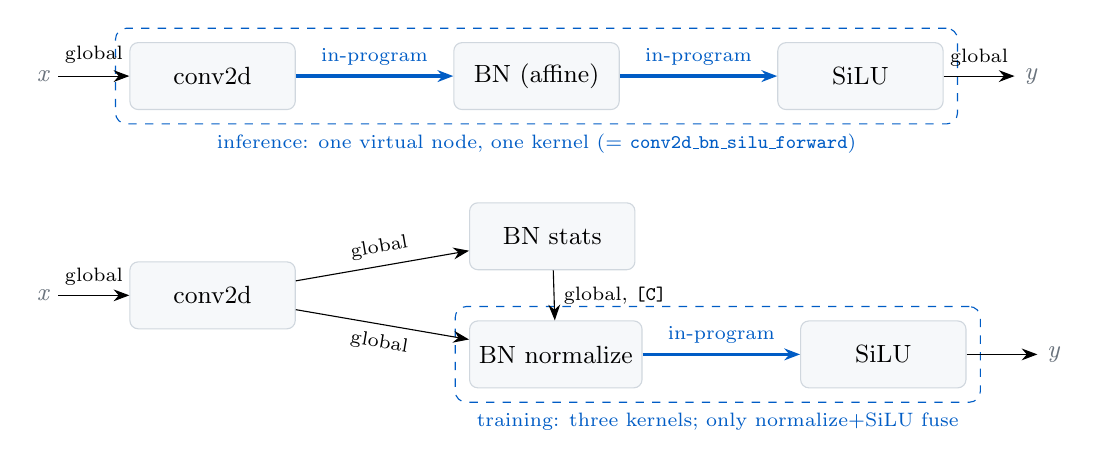
\begin{tikzpicture}[
  op/.style={draw=boxline,fill=bg,rounded corners=3pt,minimum width=2.1cm,minimum height=0.85cm,font=\small},
  io/.style={font=\small\itshape,text=cm},
  >={Stealth[length=2mm]}]
\node[io] (in) {x};
\node[op,right=0.9cm of in] (conv) {conv2d};
\node[op,right=2.0cm of conv] (bn) {BN (affine)};
\node[op,right=2.0cm of bn] (silu) {SiLU};
\node[io,right=0.9cm of silu] (out) {y};
\draw[->] (in) -- node[above=1pt,font=\scriptsize]{global} (conv);
\draw[->,very thick,attr] (conv) -- node[above,font=\scriptsize,text=attr]{in-program} (bn);
\draw[->,very thick,attr] (bn) -- node[above,font=\scriptsize,text=attr]{in-program} (silu);
\draw[->] (silu) -- node[above,font=\scriptsize]{global} (out);
\begin{scope}[on background layer]
\node[draw=attr,dashed,rounded corners=4pt,fit=(conv)(bn)(silu),inner sep=5pt,label={[font=\scriptsize,text=attr]below:inference: one virtual node, one kernel (= \texttt{conv2d\_bn\_silu\_forward})}] {};
\end{scope}

\node[io,below=2.4cm of in] (in2) {x};
\node[op,right=0.9cm of in2] (conv2) {conv2d};
\node[op,right=2.2cm of conv2,yshift=0.75cm] (st) {BN stats};
\node[op,right=2.2cm of conv2,yshift=-0.75cm] (nm) {BN normalize};
\node[op,right=2.0cm of nm] (silu2) {SiLU};
\node[io,right=0.9cm of silu2] (out2) {y};
\draw[->] (in2) -- node[above,font=\scriptsize]{global} (conv2);
\draw[->] (conv2) -- node[above,sloped,font=\scriptsize]{global} (st);
\draw[->] (conv2) -- node[below,sloped,font=\scriptsize]{global} (nm);
\draw[->] (st) -- node[right,font=\scriptsize]{global, \texttt{[C]}} (nm);
\draw[->,very thick,attr] (nm) -- node[above,font=\scriptsize,text=attr]{in-program} (silu2);
\draw[->] (silu2) -- (out2);
\begin{scope}[on background layer]
\node[draw=attr,dashed,rounded corners=4pt,fit=(nm)(silu2),inner sep=5pt,label={[font=\scriptsize,text=attr]below:training: three kernels; only normalize+SiLU fuse}] {};
\end{scope}
\end{tikzpicture}
\caption{The schedules derived in \S\ref{sec:welder-infer} and \S\ref{sec:welder-train}.}
\label{fig:schedules}
\end{figure}

\subsection{Inference, step by step}
\label{sec:welder-infer}

\textbf{Step 0: normalise the graph.} Fold BN's four per-channel parameters into
\code{scale = gamma / sqrt(var + eps)} and \code{shift = beta - scale * mean}, which
is Welder's \code{SimplifyInference}. Teenygrad already has the helper,
\code{nn::fused::prefold_bn_affine}. The \code{[C]} fold is a tiny separate node. BN
becomes a pure per-channel affine map, element-wise with two broadcast operands.

\textbf{Step 1: choose the anchor and enumerate.} \code{GraphConnecting} visits
\code{conv} first and tries connecting \code{conv->bn} in-program. The extracted
sub-graph \{conv, bn\} has \code{bn} as its output node, so tiles are enumerated on
\code{bn}'s output. Here the DSL raises its first difficulty: \code{bn}'s only
searchable axis is \code{BLOCK_HW}, while the conv's is \code{BLOCK_OW}. A fused
group has one grid, so the enumerator must pick the axis set of the node whose
\emph{body} is least flexible. That is the conv, whose decode and loop are fixed by
its declaration. The element-wise nodes adapt to any tile. So the anchor for
enumeration is the conv, and the candidates are \code{BLOCK_OW} $\in\{8, 16, 32\}$.
They describe the output tile $[1, 1, 1, b]$ of every node in the group.

\textbf{Step 2: propagate.} The seed is the group output's tile $[1,1,1,b]$, with
$b=16$. Each row is one \code{resolve_inputs} call, and each arrow is an edge
crossing:

\begin{center}
\small
\begin{tabular}{lll}
\toprule
& \textbf{with today's specs} & \textbf{with gridded axes as block 1} \\
\midrule
silu $y$ (seed) & \code{[1, 1, 1, 16]} & \code{[1, 1, 1, 16]} \\
silu $x$ & \code{[1, 1, 1, 16]} (flat, product) & \code{[1, 1, 1, 16]} \\
$\to$ bn $y$ & \code{[1, 1, 1, 16]} & \code{[1, 1, 1, 16]} \\
bn $x$ & \code{[None, None, 1, 16]} & \code{[1, 1, 1, 16]} \\
bn scale/shift & \code{[None]} (all $C$) & \code{[1]} \\
$\to$ conv $y$ & \code{[10, 8, 1, 16]} (full extent materialised) & \code{[1, 1, 1, 16]} \\
conv $x$ & \code{[None, None, None, 18]} & \code{[1, None, 3, 18]} \\
conv $w$ & --- (not in spec) & \code{[1, 3, 3, 3]} (if declared) \\
\bottomrule
\end{tabular}
\end{center}

The right-hand column is what the program actually touches. Two observations:
\begin{itemize}
\item \textbf{The left column's \code{conv y = [10, 8, 1, 16]} is harmless on its
  own.} The conv spec discards it. But a model that charged footprint per edge would
  stage a 10$\times$8$\times$16 slab for the bn$\to$conv reuse-tile when one strip is
  live.
\item \textbf{\code{bn}'s \code{BLOCK_HW} is not used at all inside the group.} The
  rider adopts the anchor's tile. \code{BLOCK_HW = 128} only describes \code{bn} as a
  standalone kernel. That is why the edge crossing must be by dim position, and why
  \code{span} was needed: without it the rank check fails at the \code{bn} row and
  propagation stops.
\end{itemize}

\textbf{Step 3: cost.} The per-program footprint is \code{x}'s region plus the
weights. BN and SiLU add two scalars and no staged tiles. Traffic is the per-tile
boundary bytes times the tile count. Computed with the corrected regions, for the
test shape:

\begin{center}
\small
\begin{tabular}{rrrrr}
\toprule
\code{BLOCK_OW} & tiles & footprint / program & traffic, fused & traffic, three kernels \\
\midrule
8  & 10{,}240 & 468 B   & 5.20 MB & 6.43 MB \\
16 & 5{,}120  & 756 B   & 4.24 MB & 5.51 MB \\
32 & 2{,}560  & 1{,}332 B & \textbf{3.76 MB} & 5.05 MB \\
\bottomrule
\end{tabular}
\end{center}

Every candidate fits, so \textsc{TopK} keeps \code{BLOCK_OW = 32}. On a 32-wide
output that is one tile per row. Fusion saves $4|y|$ ($= 1.31$~MB: BN's read and
write and SiLU's read and write of the intermediate), less the per-tile re-reads of
\code{scale}/\code{shift}. The net saving is 1.23--1.29~MB across the rows.

\textbf{Step 4: connect.} \code{conv->bn} in-program beats global, and so does
\code{bn->silu} on the next visit. The group becomes one virtual node. The rider
check must hold for each edge: \code{bn}'s grid \code{[B (Y), C, HW]} against the
anchor's \code{[B, C_OUT, OH, OW]}. It fails as literally written, for two reasons:
\begin{itemize}
\item \code{C} vs \code{C_OUT}: same dim, different name.
\item \code{HW} vs \code{(OH, OW)}: one flattened axis against two.
\end{itemize}
Since the walk crosses edges by position, the check should too. Dim~1 is dim~1
whatever each kernel calls it. A flattened rider axis is compatible with the anchor
when the anchor's tile is a valid box of it (\S\ref{sec:edges}). SiLU's single flat
axis is a subset of anything. That relaxation (positional rider matching) is the
first concrete change this graph asks of \issue{1nr.17}.

\textbf{Step 5: generate.} The fused program is the conv's prelude and loop, with
BN and SiLU applied to the carry before the store. That is
\code{conv2d_bn_silu_forward}'s \code{finish}, word for word (\S\ref{sec:prelude}).
This suggests the answer to the question \issue{1cli} left open:

\begin{note}[Proposal: a generated-loop kernel's fusion core is its carry]
For a \code{#[tile_loop(generate)]} kernel, the splice point is not ``the body minus
the store'' but ``the carry after \code{finish}''. Fusing a consumer means appending
its core to \code{finish}, with the consumer's \code{input_ident} bound to the carry:
\begin{itemize}
\item \textbf{SiLU} already has a \code{FusionCore}. Its \code{x.tensor} becomes
  \code{acc}.
\item \textbf{BN} does not have one (five inputs). Its broadcast operands would
  become rider loads keyed by the anchor's decoded index. In the hand-written
  kernel that is the \code{arange(0, 1) + tile_c_out} load in \code{finish}.
\end{itemize}
A \code{FusionCore} variant whose extra inputs are broadcast operands, each with the
anchor axis it is indexed by, would make BN spliceable. Since the macro already knows
which inputs are broadcast operands, it could emit this.
\end{note}

\subsection{What the search would really decide}
\label{sec:welder-search}

The test shape is too small to show it, so take the ResNet-stage shape
(\code{[32, 64, 56, 56]}, $3\times3$, 64$\to$64). Below is the fused
conv+BN+SiLU traffic for tiles of different \emph{shapes}, with the reduction staged
8 input channels at a time (Welder's \code{rstep}, \code{rc = 8}) for the footprint:

\begin{center}
\small
\begin{tabular}{lrrrl}
\toprule
output tile $[b, c_{\text{out}}, h, w]$ & tiles & footprint & traffic & reachable by \\
\midrule
$[1, 1, 1, 16]$  & 458{,}752 & 2.0 KB  & 7{,}432 MB & \code{conv2d_forward} \\
$[1, 1, 1, 32]$  & 229{,}376 & 3.6 KB  & 6{,}549 MB & \code{conv2d_forward} \\
$[1, 16, 1, 32]$ & 14{,}336  & 7.9 KB  & 934 MB     & \code{conv2d_bn_silu_tiled} \\
$[1, 64, 1, 56]$ & 1{,}792   & 24.0 KB & 371 MB     & \code{conv2d_bn_silu_tiled} \\
$[1, 32, 8, 8]$  & 3{,}136   & 12.4 KB & 338 MB     & needs \code{BLOCK_OH} \\
$[1, 64, 4, 28]$ & 896       & 24.2 KB & \textbf{200 MB} & needs \code{BLOCK_OH} \\
\midrule
\multicolumn{4}{l}{BN+SiLU as separate kernels add, in every row} & $+102.8$ MB ($4|y|$) \\
\bottomrule
\end{tabular}
\end{center}

This table is the strongest conclusion of the report.
\begin{itemize}
\item \textbf{Tile shape decides the traffic, not fusion.} A $1\times\text{BLOCK\_OW}$
  strip re-reads all of \code{x}'s receptive field once per output channel, so traffic
  scales with $C_{\text{out}}$. Tiling output channels divides that by the channel
  block, and tiling rows shares the halo.
\item \textbf{Fusion is worth a constant $4|y|$.} That is 1.5\% of the unfused
  total at the best \code{conv2d_forward} tile, and 34\% at the best 2-D tile. The BN+SiLU fusion only
  pays off once the conv is tiled well.
\item \textbf{The DSL bounds the search.} Welder can only enumerate the blocks a
  kernel declares. \code{conv2d_forward} offers one row of this table.
  \code{conv2d_bn_silu_tiled} offers the channel-tiled rows. The best rows need a
  \code{BLOCK_OH} (\code{#[tile_loop_tile]} accepts one blocked output axis) and a
  reduction chunk (\code{#[tile_loop]} has none).
\item \textbf{\code{../Welder} reaches the bottom rows for free.} In TE every axis is
  tileable and \code{rstep} is part of the configuration. In the DSL the equivalent
  freedom must be \emph{declared}, kernel by kernel.
\end{itemize}

\subsection{Training, step by step}
\label{sec:welder-train}

Training BN normalises with \emph{batch} statistics. For a channel $c$,
$\mu_c, \sigma_c$ need every element of channel $c$ across $B, H, W$ before any
output of that channel can be produced. (Teenygrad's BN2d training path does not do
this today, see \issue{teenygrad-fq0l}. This section assumes an NCHW stats/normalize
pair like the BN1d one in \S\ref{sec:bn}.) The graph gains a node and a fan-out:
\code{conv -> {stats, normalize}}, \code{stats -> normalize},
\code{normalize -> silu}.

\textbf{Propagate.} The seed is a SiLU tile $[1,1,1,b]$:
\begin{enumerate}
\item \textbf{normalize:} with \code{N} walked, its \code{x} resolves to
  \code{[None, 1]}, the whole channel. Even a channel-tiled normalize needs its
  channel's $\mu, \sigma$, which comes from \textbf{stats}.
\item \textbf{stats:} a \code{mean} tile \code{[1]} resolves \code{x} to every
  $(b, h, w)$ of the channel. This is the reduction-domain-is-full-extent rule of
  \S\ref{sec:bn}.
\end{enumerate}
Whatever tile the output wants, \textbf{the conv tile feeding stats is a whole
channel slab} $[B, 1, OH, OW]$.

\textbf{The candidate connections}, as traffic on the intermediate (in units of
$|y|$, excluding the conv's own input reads):

{\small
\begin{xltabular}{\linewidth}{>{\raggedright\arraybackslash}p{5.2cm}c>{\raggedright\arraybackslash}X}
\toprule
\textbf{Schedule} & \textbf{$|y|$ moved} & \textbf{Verdict} \\
\midrule
\endhead
(A) four kernels & 6 & Baseline: conv writes; stats reads; normalize reads and writes; SiLU reads and writes. \\
(B) conv $|$ stats $|$ normalize+SiLU & 4 & \textbf{What Welder picks.} normalize$\to$SiLU is element-wise with matching tiles, so it fuses exactly as in inference. \\
(C) conv+partial stats $|$ normalize+SiLU & 3 + partials & Outside the model. Each conv tile would contribute partial sums to a cross-tile reduction (atomics, or a second phase). Welder's operator-tiles are independent, and there is no edge type for ``all tiles of the producer must finish first''. \\
(D) one program per channel, all four nodes & 1 & Footprint $B\cdot OH\cdot OW\cdot 4$ per program: \textbf{40 KB} on the test shape (fits 48 KB), \textbf{392 KB} on ResNet (rejected). Even where it fits, there are only $C_{\text{out}} = 8$ programs, and the wave penalty of \S4.1 rejects it on any GPU with more SMs than that. \\
\bottomrule
\end{xltabular}
}

So the training schedule in Figure~\ref{fig:schedules} cuts at both of conv's out-edges
and saves $2|y|$, against $4|y|$ in inference. The barrier between computing a
statistic and using it is a property of the math, not of the scheduler. Welder's model
(independent tiles plus connections) represents it as a mandatory global edge.

\textbf{What the DSL would have to say for (B):}
\begin{itemize}
\item an NCHW stats kernel reducing over \code{B} and \code{HW}, which needs
  \code{reduction_axis} to become a list (\S\ref{sec:bn-train});
\item a normalize kernel with a spec that resolves per-channel operands to the
  channel tile, not full extent (\code{block = 1} or the gridded-axis rule);
\item SiLU spliced into normalize's map pass. The map pass ends in a generated store
  of the body's expression, so a consumer core can be appended to that expression,
  the multi-pass analogue of the \code{finish} proposal.
\end{itemize}

\subsection{What teenygrad needs, in order}
\label{sec:needs}

\begin{enumerate}[leftmargin=1.4em,itemsep=0.35em]
\item \textbf{Grid-decoded axes are bindings with block 1} (\S\ref{sec:conv-overestimate}).
  This fixes the 91--512$\times$ conv footprint over-estimate, resolves conv's
  \code{H} window, and makes the per-channel operands of every norm resolve to one
  channel. It removes the two-spellings gotcha.
\item \textbf{A graph-level propagate with positional edges.} Reverse-topo
  \code{resolve_inputs} plus full-extent materialisation, clamping, and re-boxing of
  flattened tiles (\S\ref{sec:edges}). Rider matching in \code{GridSpec} should then
  also be positional (\issue{1nr.17}).
\item \textbf{A graph-level \code{ConstLookup}} from each node's parameters
  (\issue{1nr.30}). Without it every window resolves to full extent.
\item \textbf{Declare what is read.} Weights, per-channel parameters through raw
  pointers, and running buffers need axes. An \code{extent} that may be an expression
  (\code{C_IN / G}) would cover conv's weight.
\item \textbf{Searchable conv tiles.} A \code{BLOCK_OH} (lift the single-blocked-axis
  limit on \code{#[tile_loop_tile]}), a \code{BLOCK_N} on the generated conv like the
  tiled variant has, and a reduction chunk on \code{#[tile_loop]} (Welder's
  \code{rstep}). \S\ref{sec:welder-search} says this is worth an order of magnitude;
  fusion is worth a third.
\item \textbf{A fusion core for generated loops} = carry after \code{finish}, plus a
  broadcast-operand-aware core so BN can be spliced (\S\ref{sec:welder-infer}).
\item \textbf{Multi-axis \code{reduce}} for NCHW training BN (\S\ref{sec:bn-train}),
  then \issue{teenygrad-fq0l} and \issue{teenygrad-1nr.18.7}.
\item \textbf{The anduin pipeline itself}: \code{schedule_graph},
  \code{Trace::trace_graph}, a profiler, and codegen, which are all \code{todo!()}
  today.
\end{enumerate}

\section{Where things live}

{\small
\begin{xltabular}{\linewidth}{>{\raggedright\arraybackslash}p{7.4cm}X}
\toprule
\textbf{Path} & \textbf{What} \\
\midrule
\endhead
\code{macros/teeny-macros/src/macros/tiled_kernel.rs} & All attribute parsing, the prelude, \code{generated_loop}, \code{generated_passes}, and the \code{tile_spec}/\code{grid_spec}/\code{fusion_core} emitters. \\
\code{core/teeny-core/src/model/tile_spec.rs} & \code{KernelTileSpec} and friends, plus \code{validate()}. \\
\code{core/teeny-core/src/model/grid_spec.rs} & \code{GridSpec}, \code{GridAxisBinding}, \code{GridDim}. \\
\code{kernels/teeny-triton/src/triton/tile.rs} & \code{Tile { tensor, mask }}. \\
\code{kernels/teeny-triton/src/fusion_core.rs} & \code{FusionCore}. \\
\code{kernels/teeny-kernels/src/graph/tile_resolve.rs} & \code{resolve_inputs}, \code{ConstLookup}, and the resolution tests per kernel family. \\
\code{kernels/teeny-kernels/src/graph/mod.rs} & \code{TritonLowering}: which kernel, which block, which spec per op. Also the spec/grid tests for conv2d and the fused kernels. \\
\code{kernels/teeny-kernels/src/graph/optimizer/anduin/} & \code{TileGraph::from_dag}; the scheduler scaffolding (\code{todo!()}). \\
\code{kernels/teeny-kernels/src/nn/conv/conv2d.rs} & \code{conv2d_forward}, \code{conv2d_bias_forward} (\code{finish} = bias), backward kernels. \\
\code{kernels/teeny-kernels/src/nn/norm/batchnorm.rs} & The four BN forward kernels (\S\ref{sec:bn}). \\
\code{kernels/teeny-kernels/src/nn/fused/} & \code{conv2d_bn_silu{,_tiled,_gemm}}, \code{prefold_bn_affine}. Microbenchmarks only, not lowered. \\
\code{kernels/teeny-kernels/tests/snapshots/} & Expanded kernel source, the ground truth for \S\ref{sec:prelude}. \\
\code{kernels/teeny-kernels/tests/test_tile_declarations.rs} & Source-parsing guard against undeclared \code{Tile} kernels. \\
\code{contributing/TiledKernelRecipe.md} & The conversion recipe (partly stale, \S\ref{sec:gotchas}). \\
\code{TILE_SCHEDULING_PIPELINE_PLAN.md} & The Roller $\to$ Welder $\to$ Rammer implementation plan. \\
\code{../Welder/ANALYSIS.md}, \code{../Welder/SHAPES.md} & Paper-to-code map of the reference implementation, and a traced conv$\to$SiLU$\to$BN through its propagation. \\
\bottomrule
\end{xltabular}
}

\section{References}

\subsection*{Papers}
\begin{itemize}
\item Y. Shi, Z. Yang, J. Xue, L. Ma, Y. Xia, Z. Miao, Y. Guo, F. Yang, L. Zhou.
  \emph{Welder: Scheduling Deep Learning Memory Access via Tile-graph.} 17th USENIX Symposium on Operating Systems Design and Implementation (OSDI '23).
  (\code{osdi23-shi.pdf})
\item H. Zhu et al. \emph{ROLLER: Fast and Efficient Tensor Compilation for Deep
  Learning.} OSDI '22. (Tile expansion, used by \textsc{EnumerateSubtiles}.)
\end{itemize}

\subsection*{Issues referenced}
\begin{center}
\small
\begin{tabularx}{\linewidth}{lX}
\toprule
\issue{teenygrad-1nr} & Welder-style TileGraph scheduler (epic). \\
\issue{1nr.15} & \code{divide_by} per instance (GroupNorm \code{C / G}). \\
\issue{1nr.17} & A fused node's grid when native grids differ (rider check). \\
\issue{1nr.18}, \issue{.18.1--.18.5} & The Tile ABI: N-D, windowed, looped, multi-blocked. \\
\issue{1nr.18.6} & \code{span}; BatchNorm2d stops being a hard boundary (PR \#103). \\
\issue{1nr.18.7} & The BatchNorm1d/3d training nodes carry their specs. \\
\issue{1nr.30} & Propagate consumes \code{TileWindow} with real const values. \\
\issue{1tl}, \issue{1tl.4--.12} & Declaring every forward kernel's axes. \\
\issue{y8aa}, \issue{3dbg}, \issue{3dp5} & The generated loop, \code{finish}, \code{init}. \\
\issue{29qp}, \issue{jpdb} & Reduced and windowed reads in the prelude. \\
\issue{3rk6.2} & \code{#[tile_reduce_pass]}, \code{walk}, the map pass. \\
\issue{1cli} & \code{FusionCore} revived (PR \#102). \\
\issue{teenygrad-fq0l} & BatchNorm2d training uses running statistics. \\
\issue{teenygrad-15k} & asin/acos/atan fail on RISC-V. \\
\bottomrule
\end{tabularx}
\end{center}


\end{document}
